\begin{center}
	\large{\textbf{BIODATA PENULIS}}
\end{center}
\begin{wrapfigure}{l}{5cm}
	\vspace{-10pt}
	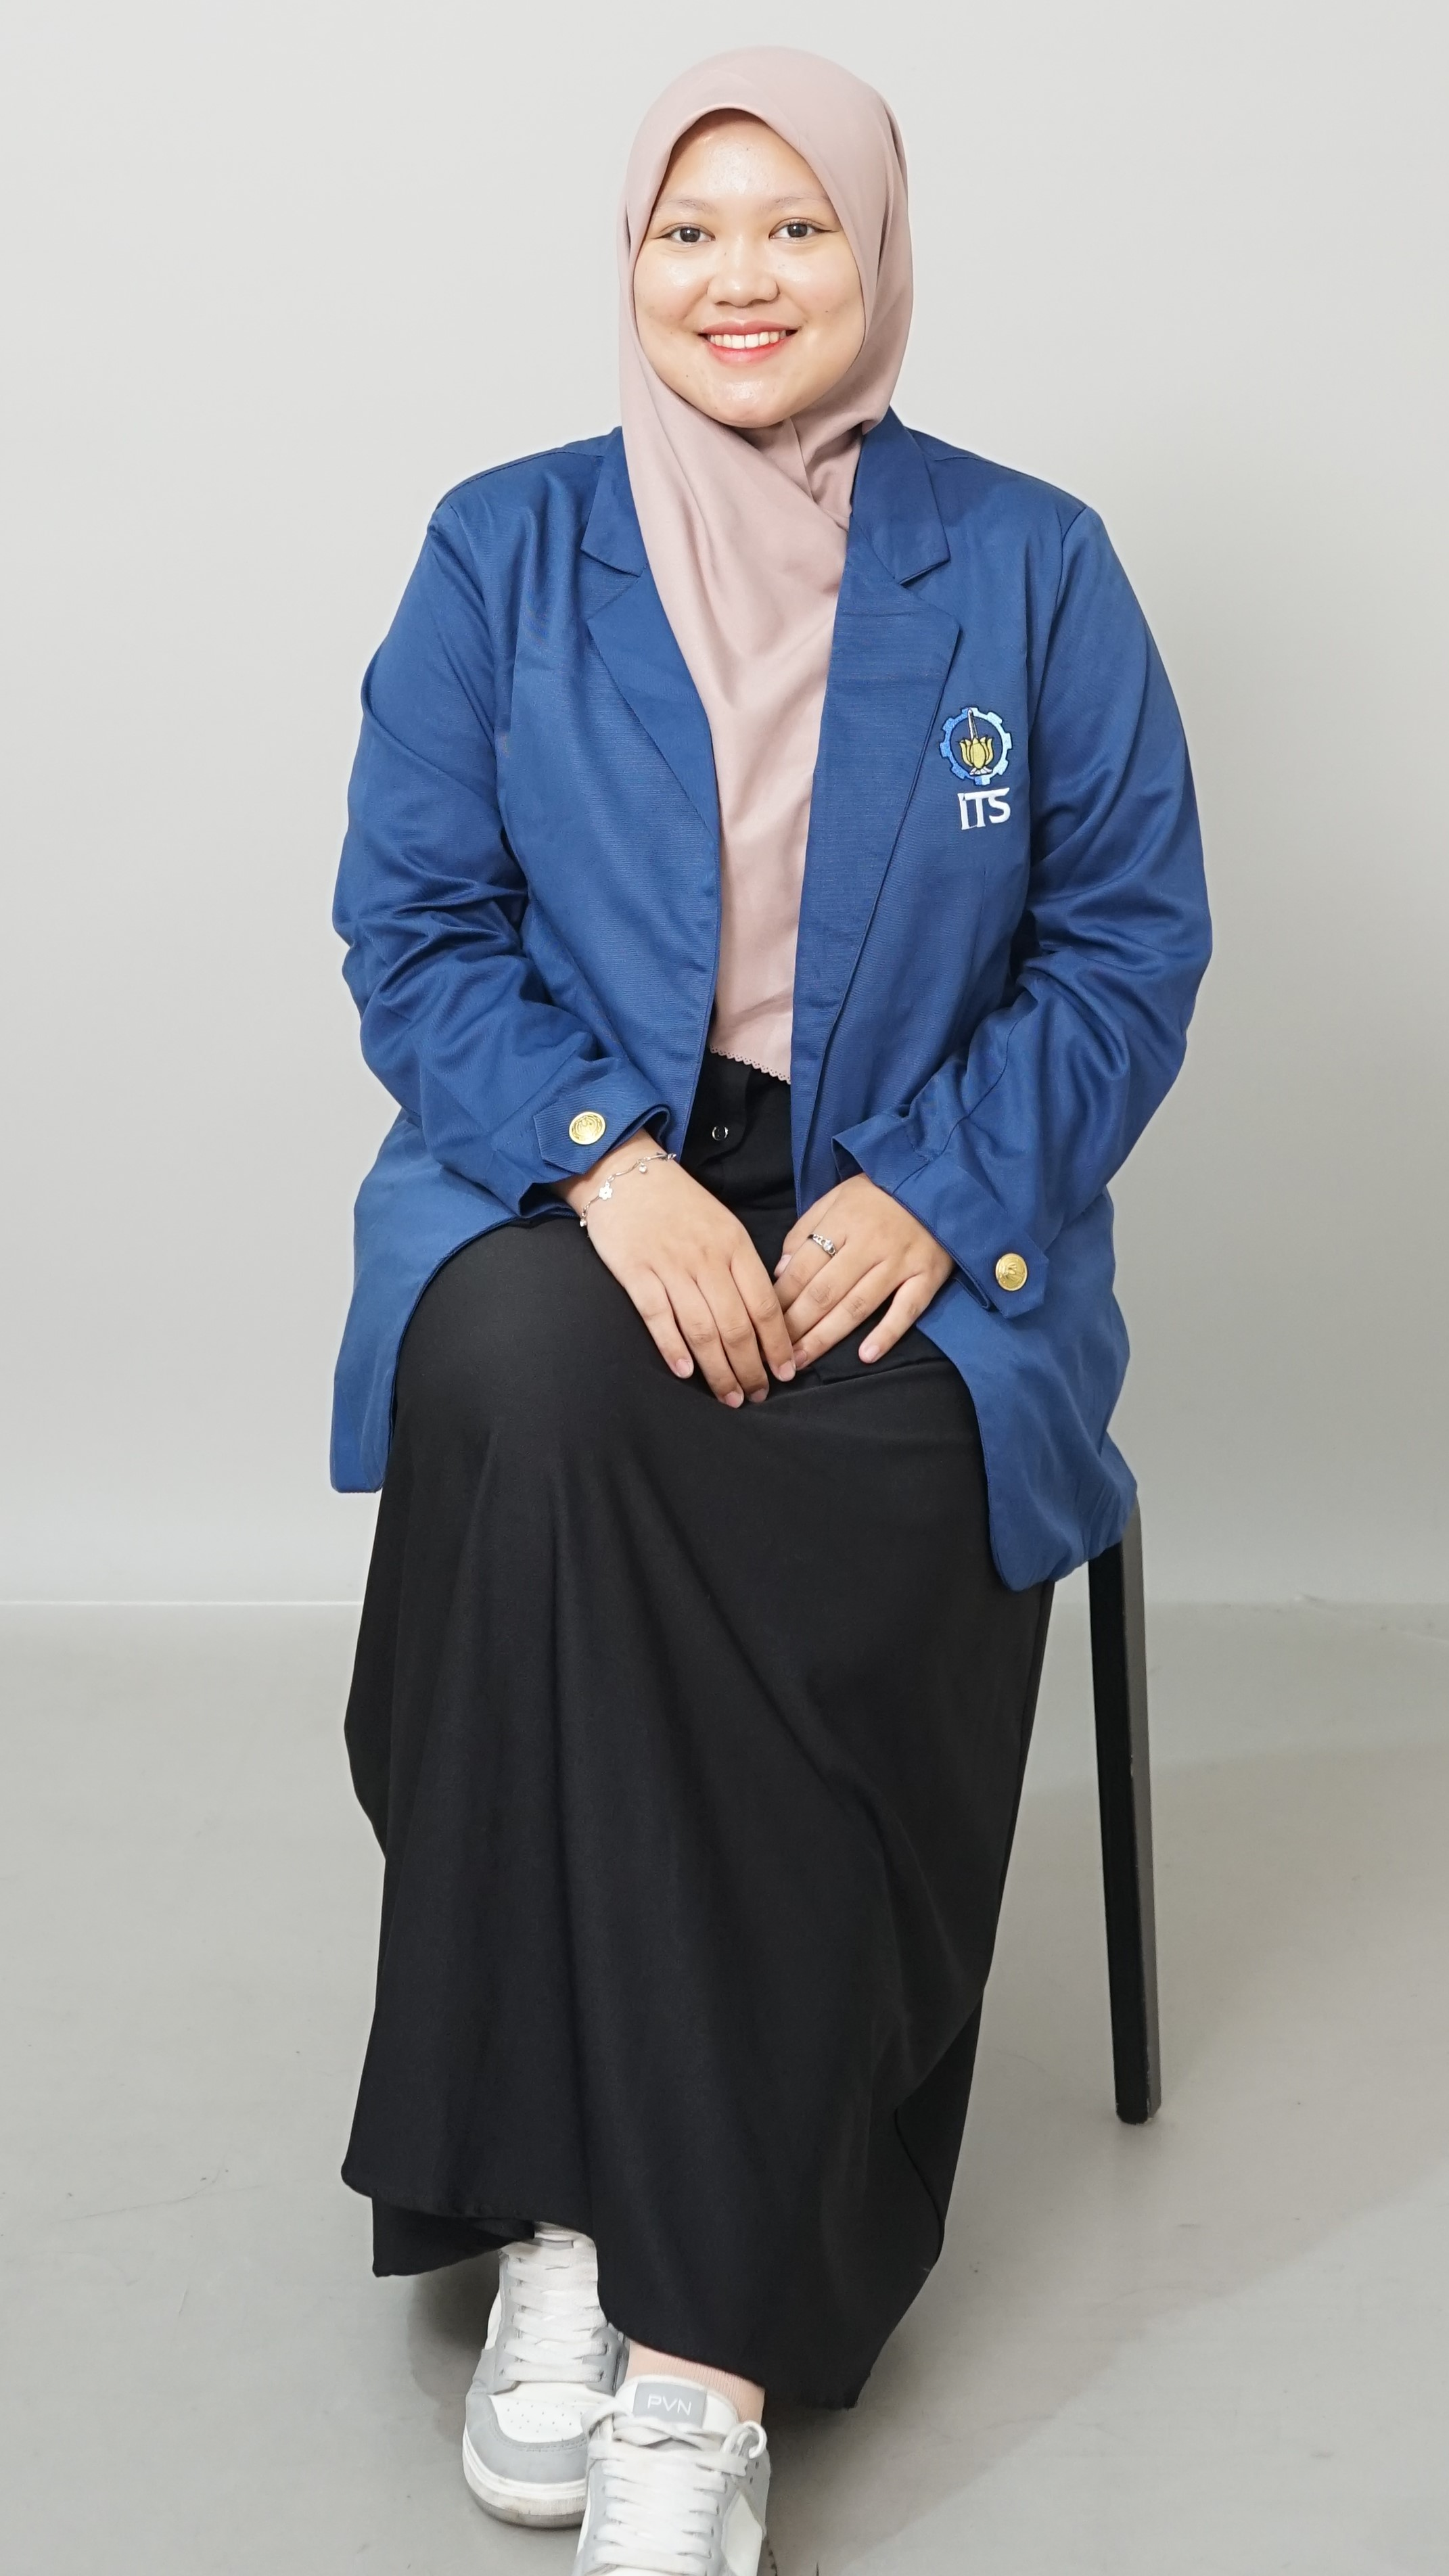
\includegraphics[width=5cm,height=9cm]{Bahan/foto_bio_Tamara_fix.jpg}
	\vspace*{-23pt}
\end{wrapfigure} 

	Penulis bernama Tamara Pingki, biasa dipanggil Tamara, lahir di Blitar, 13 Oktober 2001. Penulis merupakan anak tunggal. Penulis menempuh pendidikan formal di SDN Ngoran 2 (2008-2014), SMPN 1 Nglegok (2014-2017), SMAN 2 Blitar (2017-2019), dan S1 Pendidikan Fisika di Universitas Jember. Penulis melanjutkan ke jenjang S2 dengan mengambil bidang minat teori pada tahun 2024 melalui jalur reguler dengan NRP 6001241001.
	
	Penulis berharap kajian ini akan membawa manfaat dan dapat dikembangkan lebih lanjut oleh mahasiswa-mahasiswa fisika teori ke depannya. Jika ada pertanyaan seputar penelitian ini, penulis dapat dihubungi melalui email {tamarapingki9981@gmail.com} atau nomor ponsel 081252118246.



